%-*- program: xelatex -*-        
%-*- program: biber -*-`        
%-*- program: xelatex -*-

\documentclass[
    sigplan,
    10pt,
    review, % Note: remove the [review] option for the final document.
    natbib=false % Note: This ishere to be able to use Biber.
 ]{acmart}
\let\citename\relax

\settopmatter{printfolios=true,printccs=false,printacmref=false}

\acmConference[DLS'18]{Dynamic Languages Symposium}{November~6, 2018}{Boston, MA, USA}
\acmYear{2018}
\acmISBN{} % \acmISBN{978-x-xxxx-xxxx-x/YY/MM}
\acmDOI{} % \acmDOI{10.1145/nnnnnnn.nnnnnnn}
\startPage{1}

\setcopyright{none}

\bibliographystyle{ACM-Reference-Format}

\usepackage{booktabs}
\usepackage{subcaption}

\usepackage[
   backend=biber,
   bibencoding=utf8,
   style=numeric,
   hyperref=true,
   % citestyle=authoryear-comp,
   backref=false,
   sortlocale=en,
   url=true,
   doi=false,
   eprint=false
 ]{biblatex}
\addbibresource{biblio.bib}

\usepackage{minted}
\setminted{encoding=utf8}

\usepackage{tikz}
\usetikzlibrary{positioning}

\tikzset{
	box/.style = {
		draw = black,
        fill = white,
		rectangle,
		rounded corners = 2pt,
		text centered,
		minimum height = 5mm,
		minimum width = 10mm
	}
}

\usepackage{todonotes}
\newcommand\mb[1]{\todo[color=purple!20,size=\scriptsize]{#1}}
\newcommand\mbi[1]{\todo[color=purple!20,inline]{#1}}
\newcommand\et[1]{\todo[color=blue!20,size=\scriptsize]{#1}}
\newcommand\eti[1]{\todo[color=blue!20,inline]{#1}}

\setlength{\marginparwidth}{15mm} % Note: This is only temporary, to have notes more readable. It should be removed before submitting.

\newcommand\ignore[1]{}

\newcommand\CoqR{CoqR}

\begin{document}

\title{A Trustworthy Formalization of R} % I didn't thought much about this. Any suggestion?

\author{Martin Bodin}
\orcid{0000-0003-3588-3782}
\affiliation{
  %\position{}
  \department{Center for Mathematical Modeling}
  \institution{University of Chile}
  \streetaddress{Beauchef 851}
  \city{Santiago}
  % \state{State1}
  % \postcode{Post-Code1}
  \country{Chile}
}
\email{mbodin@dim.uchile.cl}

\author{Tom{\'a}s Diaz}
% \authornote{with author2 note}
% \orcid{nnnn-nnnn-nnnn-nnnn}
\affiliation{
  % \position{Position2a}
  \department{Computer Science Department}
  \institution{University of Chile}
  \streetaddress{Beauchef 851}
  \city{Santiago}
  % \state{State2a}
  % \postcode{Post-Code2a}
  \country{Chile}
}
\email{tdiaz@dcc.uchile.cl}

\author{{\'E}ric Tanter}
% \authornote{with author2 note}
% \orcid{nnnn-nnnn-nnnn-nnnn}
\affiliation{
  % \position{Position2a}
  \department{Computer Science Department}
  \institution{University of Chile}
  \streetaddress{Beauchef 851}
  \city{Santiago}
  % \state{State2a}
  % \postcode{Post-Code2a}
  \country{Chile}
}
\email{etanter@dcc.uchile.cl}

\begin{abstract}
\eti{update when paper is stable:}

    The R programming language is used by a large community.
    Yet, its semantics contains subtle but various corner-cases.
    This makes it difficult to fully trust an R program,
    as these corner-cases can lead to unexpected behavior.
    We believe that a Coq formalization of the language would help.

    We introduce \CoqR{}, an R interpreter (or denotational semantics) written in Coq.
    This interpreter has been related to the reference R interpreter
    GNU~R by two ways.
    First, the Coq code has been written to mimic the source code of GNU~R.
    Second, the interpreter has been extensively tested against GNU~R.
    Both these methods helped finding bugs.

    We have furthermore developed a general testing architecture
    for R interpreters.
    It guided our Coq development
    and we believe that it can be reused by other interpreters.
\end{abstract}

% %% 2012 ACM Computing Classification System (CSS) concepts
% %% Generate at 'http://dl.acm.org/ccs/ccs.cfm'.
\begin{CCSXML}
  <ccs2012>
    <concept>
      <concept_id>10003752.10010124.10010131.10010133</concept_id>
      <concept_desc>Theory of computation~Denotational semantics</concept_desc>
      <concept_significance>500</concept_significance>
    </concept>
    <concept>
      <concept_id>10011007.10011006.10011066.10011070</concept_id>
      <concept_desc>Software and its engineering~Application specific development environments</concept_desc>
      <concept_significance>300</concept_significance>
    </concept>
    <concept>
      <concept_id>10011007.10011074.10011099.10011692</concept_id>
      <concept_desc>Software and its engineering~Formal software verification</concept_desc>
      <concept_significance>100</concept_significance>
    </concept>
  </ccs2012>
\end{CCSXML}

\ccsdesc[500]{Theory of computation~Denotational semantics}
\ccsdesc[300]{Software and its engineering~Application specific development environments}
\ccsdesc[100]{Software and its engineering~Formal software verification}
% %% End of generated code

\keywords{R, Coq, Formalization, Testing}

\maketitle

\section{Introduction}
\label{sec:intro}

% R is used a lot.
The R programming language~\parencite{R, ihaka1996r, Rwebsite}
has gotten a lot of traction in recent years, being used by millions of users in areas as varied as biology and finance. This diversity among R programmers results in largely different programming styles. In fact, the language itself is community driven and reflects this diversity.

% R is complex and we need to certify R softwares.
The R programming language is meant to be both expressive and powerful,
able to express complex notions in few keystrokes.
This sometimes comes at the cost of readability. Indeed, 
the semantics of R is subtle and contains numerous corner cases that can result in unexpected behavior. 

The reasons for these corner cases are numerous, ranging from backward compatibility to the desire to accommodate the use of R as both a traditional programming language and an interactive shell.
Even a feature as basic as function calls can be the source of surprises in R. 
Indeed, there are many ways to call a function, and in particular there are two ways to provide an argument: either by position or by name.\footnote{
    To simplify, here we ignore the \mintinline{R}{...} notation
    as well as default arguments, which both have non-trivial interactions with the function call mechanisms.}

Figure~\ref{fig:calls} defines a function \mintinline{R}{f} that concatenates its three arguments. The first call associates arguments by position, and the second by name. The third call mixes both mechanisms. But in R, 
association by name can be made {\em by prefix}:
observe that the third call associates \mintinline{R}{d} to \mintinline{R}{de}
because it is the only argument whose name starts with \mintinline{R}{d}.
If more than one argument matches by prefix,
then R rejects the call and throws an error,
as in the fifth call in Figure~\ref{fig:calls}.
However, exact matches are not counted in this process:
in the fourth call,
the name \mintinline{R}{ab} is an exact match
and thus only the argument \mintinline{R}{abc}
is left to be associated to \mintinline{R}{a},
leading to no error thrown.

\begin{figure}[t]
\begin{minted}{R}
f <- function (abc, ab, de) { c (abc, ab, de) }
f(1, 2, 3)           # By position
f(de=3, abc=1, ab=2) # By name
f(1, d=3, 2)         # Mixed
f(3, a=1, ab=2)      # a is associated to abc
f(a=3, 1, 2)         # error: several prefixes
\end{minted}
\caption{Exploring function calls in R.}
\label{fig:calls}
\end{figure}

Such subtle behaviors are numerous in R~\parencite{RInferno}.
Debugging tools exist~\parencite{mcpherson2014},
but they cannot always compensate for the complex semantics of R.
Consequently, surprising bugs occur in R programs
and fully trusting such programs can be difficult.

% We need a formalization of the language.
Formal methods offer a solution to the trust issue:
proof assistants such as Coq~\parencite{Coq} enable us
to formally prove program properties with a high amount of trust.
But to formally prove that an R program meets its specification,
we first need a formal semantics of R. \et{mention the on-going spec effort and its limits} 
In particular, the formal semantics should account for all the subtle cases of the R semantics, such as function call conventions described above, implicit type conversions, and so on.
This is necessary because these corner cases are indeed a typical place were bugs appear and are hard to track. 
A complete semantics for the full R language will inevitably be complex,
because of the large amount of such corner cases.

% This formalization is quite large, and we need to certify it.
This complexity in turn raises a meta-trust issue: 
how can a large semantics (and consequently the proofs made from it)
be trusted?
The approach we take in this work
\eti{in line with prior work on JavaScript (lambdaJS in particular, can we say the same of JSCert?), also C? what else?}
\mbi{
    We can say the same for lambdaJS/ES5 and KJS, although we are then only talking about testing and not line-to-line correspondence.
    We also can for JSCert, although it was tested against test suites and not a reference interpreter.
    I don't think that we can say the same for CompCert or Formalin, as they only considered the C specification.
    Maybe CompCertS falls into this category as it tried to mimic the behavior of real-world compilers, but I don't remember that it was actually tested.}
is to relate the formal semantics to the reference interpreter of R, GNU~R~\parencite{Rwebsite}. In the absence of a standardized formal semantics, GNU~R is the reference point that defines what the R language really is.
Being able to relate the formalism to trust sources is a crucial aspect of the formalization process, and often requires a large amount of work
to be done properly~\parencite{leroy2014pip}.

\paragraph{Contributions.} 
We present \CoqR{}, a trustworthy formalization of the R programming language in the Coq proof assistant.
The formalization is a denotational semantics, in the form of an interpreter.
This interpreter is trustworthy because we have followed two complementary techniques to maximize trust, inspired by the JSCert project~\parencite{popl14jscert}.
First, the Coq interpreter has been written using a monadic encoding that allows for a direct eyeball correspondence with the C source code of GNU~R.
Second, we have extensively tested the interpreter against the R reference interpreter.\et{using the standard test suites? and additional ones?}\mb{I think that we can cite the FastR paper at this stage~\parencite{kalibera2014fast}: they talk about their test suite.}
To this end, we have developed a testing framework that streamlines the process of running both the Coq interpreter and GNU~R on a set of test cases and report on mismatches and errors.
We report on the process of scaling up our interpreter in order to be able to import existing R libraries.

% Given the size of our formalization,
% we consider this part to be the most important of our contributions.

% The development presented here, including the Coq interpreter, the testing framework, and the tests, is available online at:\\
% \url{https://github.com/Mbodin/proveR/releases/tag/DLS2018}\todo{make this tag exist on Github}.

% % Contributions.
% We introduce \CoqR{}

% a formalization of the R programming language in the Coq proof assistant.
% This is a continuation of a previous work~\parencite{CoqRCoqPL},
% \mb{Political choice here: is it a good idea to cite this previous work?}\et{no, skip - this wasn't a technical result, just a progress report/position paper}
% in which we formalised a small core of the R language.
% The additional contribution of this paper is the additional
% of a non-trivial quantity of R features,
% which enabled us to import R libraries.
%
%
% This two-factors method is very close to the one of JSCert,
% which we discuss in Section~\ref{sec:related:work}.



% Outlines.
\eti{update when paper is stable:}
This paper is organized as follows.
Section~\ref{sec:coq:interp} presents the Coq denotational semantics.
In particular, Section~\ref{sec:eyeball:closeness} presents
how this semantics is syntactically close to the C source code of R.
Section~\ref{sec:testing:architecture} then presents our testing architecture.
Not only this architecture is used as a way to relate our semantics
with R reference interpreter,
it also provided immediate benefits during the development of the semantics.
Section~\ref{sec:driving:development} presents these benefits.
The testing results are shown in Section~\ref{sec:test:results}.
Finally, Section~\ref{sec:proofs} presents some proofs that have been done
using our language formalization.

\section{Coq Interpreter}
\label{sec:coq:interp}

Our semantics of R is presented on the form of an interpreter
and is thus denotational.
Denotational semantics are usually not the best fit for Coq proofs---%
inductive operational semantics are usually more adapted---%
but it comes with a crucial advantage:
it can be run, and thus tested.

In this section, we show how we define the Coq interpreter in order to achieve the first of the two mechanisms in place for trust, namely the eyeball correspondence with the GNU~R interpreter.

\subsection{Bridging the Gap between C and Coq}
\label{sec:monad}

The basic principle of eyeball correspondence is that every one or two lines of the Coq interpreter should correspond to one or two lines of the C reference interpreter.

Of course, achieving a close correspondence between C and Coq versions of the same program is challenging, because C and Coq are widely different programming languages:
Coq is purely functional
whilst global side-effects are frequent in C.
Furthermore, Coq is designed to reject any function
whose behavior is not entirely defined
(it is for instance impossible to miss a case in a pattern-matching),
whilst C is known for its undefined behaviors.
Finally, contrary to C,
Coq programs are required to terminate.


\begin{figure}[t]
\begin{minted}{Coq}
Inductive result (A : Type) :=
  | result_success : state -> A -> result A
  | result_error : state -> string -> result A
  | result_longjump : state -> context -> result A
  | result_impossible : state -> string -> result A
  | result_not_implemented : string -> result A
  | result_bottom : state -> result A.
\end{minted}
\caption{The result monad.}
\label{fig:result}
\end{figure}

In order to limit the impact that these differences can have on the eyeball correspondence, we introduce a {\em result monad}, which combines both the state, error, and fuel monads (Figure~\ref{fig:result}), and allows us to program in Coq ``as if it were C''. 
\et{add some basic introductory level stuff on monads, and each of these...}
More precisely, the result monad features the following constructors:\footnote{The result monad is similar to the one used in the JSExplain project~\parencite{JSExplain}, which aims at defining a JavaScript interpreter in Coq, readable by non-specialists. 
}
\begin{itemize}
\item The main constructor is \mintinline{Coq}{result_success}, used when a computation is successful.
In addition to the result (of type \mintinline{Coq}{A} in the definition),
it carries the global state (of type \mintinline{Coq}{state}). (We describe the representation of state later on in this section.)
%
\item The constructor \mintinline{Coq}{result_error} is meant to catch
errors thrown by GNU~R, for instance an R runtime typing error:
these errors are not catchable and immediately end the execution.
A \mintinline{Coq}{string} is provided to help the debugging process.
%
\item The constructor \mintinline{Coq}{result_longjump}
appears in constructs involving non-local jumps like \mintinline{R}{break}
or \mintinline{R}{return}.
We do not give much details about this constructor in this paper.\et{why not?}\mb{If we have space, I can add some details. But it really boils down to a specific C behavior that is not that much used in the interpreter (mainly in one place in function calls).}
%
\item Unspecified C behaviors are translated into \mintinline{Coq}{result_impossible}. This typically includes dereferencing an invalid pointer.
Getting this result immediately ends the Coq interpreter: it is meant to be unreachable. Observing such a result means that a bug in GNU~R has been found.\et{has this happened? I guess not}\mb{No it hasn't. What I meant but that is that in \CoqR{}, such a mistake always result in an error, whilst in GNU~R, this could result in a silent error due to compiler optimizations: we are in theory able to catch bugs that direct testing on GNU~R wouldn't be able to catch.}
%
\item Given the size of the interpreter\et{not mentioned before},
it is important to be able to execute it without it being complete.
The \mintinline{Coq}{result_not_implemented} is thus important
for the development, and is treated specifically in our testing framework.
%
\item Finally, \mintinline{Coq}{result_bottom} is returned
to end the execution when reaching the maximum number of executed instructions
(also called \emph{fuel}). This is meant to artificially make our interpreter terminate, despite the fact that the interpreted R program may not.
\end{itemize}

The result monad is associated with a monadic binder,
written \mintinline{Coq}{let%success}.
This binder expects its argument to evaluate to a result of the form
\mintinline{Coq}{result_success}. If so, it binds the carried result to a name, and transparently propagates the possibly-updated state.
All other kinds of results are transparently propagated to the top-level. This obliviousness to global state, errors and non-termination is what enables a close correspondence between a program written in both languages.

% We believe that this helps to find bugs in \CoqR{}
% and to convey trust to the overall R semantics.

\subsection{Eyeball Correspondence}
\label{sec:eyeball:closeness}

\begin{figure*}[t]
    \centering{}
\begin{subfigure}{.54\textwidth}
\begin{minted}{C}
EXP* do_attr (EXP* call, EXP* op,
              EXP* args, EXP* env){
  EXP* argList, car, ans;
  /* ... */
  int nargs = R_length (args);
  argList = matchArgs (do_attr_formals, args, call);
  PROTECT (argList);
  if (nargs < 2 || nargs > 3)
    error ("Wrong argument count.");
  car = CAR (argList);
  /* ... */
  return ans;
}
\end{minted}
    \caption{original C function}
    \label{fig:c:do_attr}
\end{subfigure}
\begin{subfigure}{.45\textwidth}
\begin{minted}{Coq}
Definition do_attr globals runs S
    (call op args env : EXP_pointer) :=
  let%success nargs :=
    R_length globals runs S args using S in
  let%success argList :=
    matchArgs globals runs S
      do_attr_formals args call using S in
  if nargs <? 2 || nargs >? 3 then
    result_error S "Wrong argument count."
  else
    read%list car, _, _ := argList using S in
    (* ... *)
    result_success S ans.
\end{minted}
    \caption{Coq translation}
    \label{fig:coq:do_attr}
\end{subfigure}
    \caption{Original C function and Coq translation of \mintinline{C}{do_attr}}
    \label{fig:do_attr}
\end{figure*}


% % Definition of the line-to-line correspondence.
% One key specificity of this interpreter is that it has been designed
% to be similar to the original C source code of GNU~R.
% More precisely, they are related by a line-to-line correspondence
% (also called \emph{eyeball closeness})\et{is closeness a standard term here? (eyeball correspondence sounds better to me)}:
% every one or two lines of our interpreter
% correspond to one or two lines of the reference interpreter.
% %

By developing \CoqR{} as a monadic interpreter using the result monad introduced above, we are able to achieve an eyeball correspondence between the C and Coq interpreters. This correspondence is extremely helpful during development:
whenever a bug is encountered while testing, we localize the function responsible for the bug and then check the line-to-line correspondence.
Such checks are quick and easy to perform, often leading to a quick fix of \CoqR{}.
%

Figure~\ref{fig:do_attr} shows an example of the eyeball correspondence that can be achieved using the result monad. Figure~\ref{fig:c:do_attr} shows a C function, and Figure~\ref{fig:coq:do_attr} its Coq translation.
The binder \mintinline{Coq}{let%success} is used when calling a function. 
For instance, the calls to \mintinline{Coq}{R_length}
and \mintinline{Coq}{matchArgs}
may return an unsuccessful result,
and the code afterwards will only be executed if the result has been successful.

\et{walk the reader through the correspondence: comparison operators, raising an error, returning the final result. } 

The other differences that one can observe are several arguments that are systematically passed to each function (\mintinline{Coq}{globals}, \mintinline{Coq}{runs}, and \mintinline{Coq}{S}), as well as the use of 
\mintinline{Coq}{read%list} 
instead of \mintinline{C}{CAR} in the C version, and the fact that the use of the \mintinline{C}{PROTECT} macro is missing from the Coq version. We clarify each of these points in the following subsections.

% The \mintinline{Coq}{S} argument and the use 
% are related to the modeling of the heap, discussed in Section~\ref{sec:coq:structure}.

% The \mintinline{Coq}{globals} argument is discussed in Section~\ref{sec:coq:structure}.

% The \mintinline{Coq}{runs} argument is related to dealing with non-termination, and is discussed in Section~\ref{sec:fuel}.



\subsection{Modeling the Heap}
\label{sec:heap}

\begin{figure}
    \centering{}
    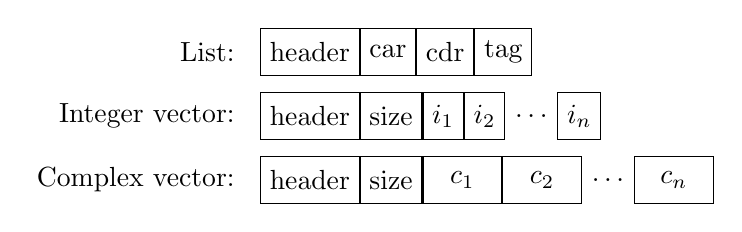
\begin{tikzpicture}
        \node [draw = black, rectangle, minimum height = 6mm, anchor = base] (hlist) {header} ;
        \node [draw = black, rectangle, minimum height = 6mm, anchor = base, right = 0pt of hlist] (car) {car} ;
        \node [draw = black, rectangle, minimum height = 6mm, anchor = base, right = 0pt of car] (cdr) {cdr} ;
        \node [draw = black, rectangle, minimum height = 6mm, anchor = base, right = 0pt of cdr] (tag) {tag} ;
        \node [left = 2mm of hlist] (nlist) {List:} ;

        \node [draw = black, rectangle, minimum height = 6mm, anchor = base, below = 2mm of hlist] (hvector1) {header} ;
        \node [draw = black, rectangle, minimum height = 6mm, anchor = base, right = 0pt of hvector1] (size1) {size} ;
        \node [draw = black, rectangle, minimum height = 6mm, anchor = base, right = 0pt of size1] (i1) {\(i_1\)} ;
        \node [draw = black, rectangle, minimum height = 6mm, anchor = base, right = 0pt of i1] (i2) {\(i_2\)} ;
        \node [anchor = base, right = 0pt of i2] (i3) {\(\ldots\)} ;
        \node [draw = black, rectangle, minimum height = 6mm, anchor = base, right = 0pt of i3] (in) {\(i_n\)} ;
        \node [left = 2mm of hvector1] (nvector1) {Integer vector:} ;

        \node [draw = black, rectangle, minimum height = 6mm, anchor = base, below = 2mm of hvector1] (hvector2) {header} ;
        \node [draw = black, rectangle, minimum height = 6mm, anchor = base, right = 0pt of hvector2] (size2) {size} ;
        \node [draw = black, rectangle, minimum height = 6mm, minimum width = 1cm, anchor = base, right = 0pt of size2] (c1) {\(c_1\)} ;
        \node [draw = black, rectangle, minimum height = 6mm, minimum width = 1cm, anchor = base, right = 0pt of c1] (c2) {\(c_2\)} ;
        \node [anchor = base, right = 0pt of c2] (c3) {\(\ldots\)} ;
        \node [draw = black, rectangle, minimum height = 6mm, minimum width = 1cm, anchor = base, right = 0pt of c3] (cn) {\(c_n\)} ;
        \node [left = 2mm of hvector2] (nvector2) {Complex vector:} ;
    \end{tikzpicture}
    \caption{Basic language elements in memory}
    \label{fig:basic:language:elements}
\end{figure}

% Basic language elements.
We now describe how we modeled GNU~R's heap.
Although the underlying language is C,
GNU~R has been designed with a specific structure in mind~\parencite{R}.
Almost all objects manipulated by the interpreter
are called \emph{basic language elements},
or \mintinline{C}{EXP} in C.
Each of them are composed of a header and some data.
%
The header stores the type of the basic language element,
a list of attributes,
as well as several mostly-boolean informations
(for instance whether it can be safely updated in place).
There are \(24\) different types of basic language elements in R,
\(9\) of which being different kinds of vectors.
%
The stored data depends on the type of the element.
For instance, lists contain three pointers:
one to the first element (named \mintinline{Coq}{car}),
to the queue of the list (\mintinline{Coq}{cdr}),
and to an optional name for the first element (\mintinline{Coq}{tag}).
Vectors store their length,
followed by a C array in memory.
The size of this array depends both of its length
and the type of vector.
Figure~\ref{fig:basic:language:elements} illustrates this
with integer and complex vectors
(complexes are composed of two floats).
%
The way memory is used in C
makes it easy to unguardedly access a cell out of bounds,
which would lead to an undefined behavior.



% Guarded accesses in Coq to represent unguarded accesses in C.
This is an issue,
as we cannot directly translate unguarded C accesses into Coq:
we need a model of the heap.
Figure~\ref{fig:EXP} shows how we defined \mintinline{Coq}{EXP} in Coq.
Basic language elements are records storing a header
and data,
which in turn is defined as a sum type.
For instance, lists are defined by three pointers.
Vectors are records storing their length and a list:
in Coq, the data of vector is stored directly in the \mintinline{Coq}{EXP} structure
and not following it in memory as in C.

\begin{figure}
\begin{minted}{Coq}
Record ListStruct := make_ListStruct {
    lSist_carval : EXP_pointer ;
    lSist_cdrval : EXP_pointer ;
    lSist_tagval : EXP_pointer
  }.

Record Vector_EXP (A : Type) := make_Vector_EXP {
    Vector_length : nat ;
    Vector_data :> list A
  }.

Inductive EXPData :=
  | listExp : ListStruct -> EXPData
  | envExp : EnvStruct -> EXPData
  | EXP_VectorInteger : Vector_EXP int -> EXPData
  | EXP_VectorComplex : Vector_EXP complex -> EXPData
  (* ... *).
Coercion listExp : ListStruct >-> EXPData.
Coercion envExp : EnvStruct >-> EXPData.
(* ... *)

Record EXP := make_EXP {
    EXP_header :> EXPHeader ;
    EXP_data :> EXPdata
  }.
\end{minted}
    \caption{Basic language elements (\mintinline{C}{EXP}) in Coq}
    \label{fig:EXP}
\end{figure}

% About the use of coercions.
To ease readability, coercions have been used extensively.
Coercion is a mechanism to mark some constructors as implicit.
For instance, if Coq expects a \mintinline{Coq}{EXPData}
and is given a \mintinline{Coq}{ListStruct},
then the constructor \mintinline{Coq}{listExp} will be implicitly called
thanks to the corresponding line in Figure~\ref{fig:EXP}.
In the context of \CoqR{},
this is more than a simple syntactic notation
as it helps the line-to-line correspondence
by hiding what is not present in C:
if one points to either a list or an environment,
the C notation to access its list or its environment is the same.
%
Of course, this implicit notation is only one-way:
given a \mintinline{Coq}{ListStruct},
we can convert it into an \mintinline{Coq}{EXPData},
but to perform the converse, we have to pattern-match
on the shape of the \mintinline{Coq}{EXPData}.
%
This pattern-matching is performed by specific monadic binders.
For instance in Figure~\ref{fig:coq:do_attr}, \mintinline{Coq}{read%list}
gets the \mintinline{Coq}{EXP} stored in the state \mintinline{Coq}{S}
and pointed by \mintinline{Coq}{argList},
then pattern-matches it as a list,
extracting the \mintinline{Coq}{car}, \mintinline{Coq}{cdr},
and \mintinline{Coq}{tag} fields.
If the pointer is not in the domain of the state \mintinline{Coq}{S}
or if the associated \mintinline{Coq}{EXP} object is not a list,
then \mintinline{Coq}{result_impossible} is returned:
this corresponds to an undefined behavior in C
(dereferencing an invalid pointer or accessing the wrong projection of a \mintinline{C}{union}).
The accesses in Coq are thus guarded by monadic binders,
whilst closely mimicking the unguarded accesses of C.


% Not modeling this part enabled us to focus on the computational part.
%
%
% At this stage, the reader should be able
% to compare the C and Coq programs of Figure~\ref{fig:do_attr}
% line by line.
% The rest of \CoqR{} was similarly defined.

\subsection{Dealing with Global Variables}
\label{sec:globals}

% Initialization of R and global variables.
The GNU~R interpreter features over \(80\) global variables that need initialization, and are subsequently unchanged. 
The initialization of these internal variables
actually represents a large portion of the source code.
Even before importing any libraries, a lot of basic language elements
are created and stored in global variables.

For instance, the often-used variable \mintinline{C}{R_NilValue}
is set to be a list whose \mintinline{C}{car}, \mintinline{C}{cdr},
and \mintinline{C}{tag} fields point to \mintinline{C}{R_NilValue} itself.
This element is used instead of the \mintinline{C}{NULL} pointer
to mark any non-present element. Another important global variable is 
\mintinline{C}{R_FunTab}, which is the {\em symbol table} that maps operation and function names to C functions implementing them. (We exploit this structuring of the interpreter for building \CoqR{} in an incremental manner---see Section~\ref{sec:coq:structure}.)

%
The initialization of global variable is fairly subtle. Most initializations perform local computations, calling core functions.
To avoid this circular dependency---which Coq would not accept---one could parametrize each core function by the value of the global variables it uses.
This would however not scale, considering the size of the project and the number of global variables involved.
%
Instead, we parameterize each function of \CoqR{} by a single \mintinline{Coq}{globals} environment, which is a mapping from a definite set of global variables to \mintinline{Coq}{EXP_pointer}. This additional argument can be seen in the Coq code of Figure~\ref{fig:coq:do_attr}: it is passed along at each call site.

To make definitions more convenient, we use coercions to make Coq implicitly perform a lookup in the \mintinline{Coq}{globals} environment whenever a global variable is read. Therefore, accessing global variables is transparent, as illustrated by the use of \mintinline{C}{do_attr_formals} in Figure~\ref{fig:coq:do_attr}.


\begin{figure*}
    \centering{}
\begin{subfigure}{.5\textwidth}
\begin{minted}{C}
  static EXP* do_attr_formals = NULL;
  if (do_attr_formals == NULL)
    do_attr_formals =
      allocFormalsList2 (install ("x"),
                         install ("which"));
\end{minted}
    \caption{C snippet}
    \label{fig:c:do_attr:formals}
\end{subfigure}
\begin{subfigure}{.49\textwidth}
\begin{minted}{Coq}
Definition do_attr_init globals runs S :=
  let%success x :=
    install globals runs S "x" using S in
  let%success which :=
    install globals runs S "which" using S in
  allocFormalsList2 globals S x which.
\end{minted}
    \caption{Coq translation}
    \label{fig:coq:do_attr:formals}
\end{subfigure}
    \caption{Another snippet of \mintinline{C}{do_attr} and its Coq translation}
    \label{fig:do_attr:formals}
\end{figure*}

% Static global variables.
\paragraph{Hidden global variables.} In fact \mintinline{C}{do_attr_formals} is a {\em hidden} global variable, introduced locally with the C \mintinline{C}{static} keyword inside the \mintinline{C}{do_attr} function. Such a variable is persistent across calls, just like a standard global variable.

In place of the first commented-out part in Figure~\ref{fig:c:do_attr}, the code actually defines the \mintinline{C}{static} variable \mintinline{C}{do_attr_formals}, as shown in Figure~\ref{fig:c:do_attr:formals}. Upon the first call of \mintinline{C}{do_attr}, the variable \mintinline{C}{do_attr_formals} is initialized by a basic language element. The value is kept across calls in order to avoid a costly reallocate at each call.
%
Observe that this pattern exactly follows the scheme of the other global variables: the variable is initialized once, and then never changes. Consequently, we treat such a \mintinline{C}{static} variable just like a global variable. We extracted out the part of \mintinline{C}{do_attr} that performs initialization, shown in Figure~\ref{fig:coq:do_attr:formals}.
This code is executed after the standard global variables are initialized.\et{what if the initialization of a static var uses some argument of the first call? does it ever happen?}\mb{I've never seen it. In such a case, I just add these variables in the state (this already happenned, but is rare).}


\subsection{Dealing with Non-Termination}
\label{sec:fuel}
% Structuring the fuel.
Another additional argument present in Figure~\ref{fig:coq:do_attr}
is the \mintinline{Coq}{runs} argument.
This argument aims at factorizing the fuel given to Coq function
to make them artificially terminate.
The usual way to do this is to make each function check whether its fuel
reached \(0\), and if so return \mintinline{Coq}{result_bottom}.
This is not practical as it repeats the same code
and breaks with the line-to-line correspondence
(this operation not being done in C).
%
We solved this issue by adopting the same method than in JSCert:
instead of a fuel argument, each function takes a record \mintinline{Coq}{runs}.
This record stores all recursive functions as its projections.
Each recursive call in C are then translated by calling
the corresponding projection of the record,
as in a regular fixed-point combinator.
\mb{I guess that this paragraph could be improved a lot\ldots}
Once all functions have been defined,
one can then define a function \mintinline{Coq}{runs} taking some fuel:
at each step, its projections are functions taking a \mintinline{Coq}{runs}
with less fuel as argument;
when reaching \(0\), all its projections systematically return \mintinline{Coq}{result_bottom}.
Figure~\ref{fig:runs} shows its Coq definition.
%
\mb{Maybe we just don't want to speak about this:}
\mbi{
Note that the symbol table has to be one of the projections of \mintinline{Coq}{runs},
otherwise a user could make the Coq interpreter loop by giving as argument\ldots not clear,actually.
}
%
This structure only needs one pattern-matching on fuel
in the whole \CoqR{} interpreter.
It is thus a scalable way to organize our Coq project.

\begin{figure}
\begin{minted}{Coq}
Fixpoint runs max_step globals :=
  match max_step with
  | O => {|
      runs_while_loop := fun _ S _ _ _ =>
        result_bottom S ;
      runs_eval := fun S _ _ =>
        result_bottom S ;
      (* ... *) |}
  | S n => {|
      runs_while_loop := fun A S (a : A) expr stat =>
        while_loop globals (runs n) A S a expr stat ;
      runs_eval := fun S e rho =>
        eval globals (runs n) S e rho ;
      (* ... *) |}
  end.
\end{minted}
    \caption{Definition of \mintinline{Coq}{runs} in Coq}
    \label{fig:runs}
\end{figure}


\subsection{Limitations}
% About garbage collection.
The use of the \mintinline{C}{PROTECT} macro in Figure~\ref{fig:c:do_attr} is missing in the Coq translation. This macro use performs a garbage collecting action, namely it saves the object \mintinline{C}{argList} from garbage collection.
At this stage, we chose not to model the garbage collection aspect of GNU~R in \CoqR{}. Indeed, garbage collection adds complexity to the interpreter, but is not supposed to affect the result of any computation. For now, we focus on the computational part of GNU~R.

% Ignored aspects.
% As stated in Section~\ref{sec:eyeball:closeness},
% we chose to ignore some aspects of the source code of GNU~R.
% All garbage collection commands have been formalized out.
Additionally, \CoqR{} only considers ASCII strings, and hence does not support various locales and character encodings supported by R. 
More generally, \CoqR{} ignores any possibility to dynamically
parametrize the behavior of the interpreter using options
stored the shell environment.

\mb{Are there other things we should mention?}

Note that the eyeball correspondence between GNU~R and \CoqR{} would pay off in the future if one wants to extend \CoqR{} to account some of these features, such as garbage collection.



\subsection{Incremental Development of \CoqR{}}
\label{sec:coq:structure}

R is by no means a small language.
As a result, the \CoqR{} project spans over 18,000 lines of Coq definitions.
This is larger than in the JSCert project~\parencite{popl14jscert}.\et{ref + how large is JSCert?}\mb{We already quote it several times in the paper: isn't it too much?}
\mbi{For the statistics: \CoqR{} is 18,000 lines of Coq definitions + 1500 lines of Coq proofs.
    JSCert is 12,500 lines of Coq definitions + 5,000 lines of Coq proofs. Both according to \texttt{coqwc}.
    It is difficult to compare these figures, but I find the comparizon with JSCert impressive.}
Therefore, for pragmatical reasons, it was important to be able to proceed incrementally in the development of \CoqR{}. We hence had to identify a minimal core of R to support initially, and then incrementally extend \CoqR{}. To this end, we exploited the fact that GNU~R is structured around a huge {\em symbol table} that contains all functions present in the initial environment of R, whose code is written natively in C.

\begin{figure}
\begin{minted}{C}
FUNTAB R_FunTab[] = {
  {"if",        do_if,       2,  true,  false},
  {"while",     do_while,    2,  true,  false},
  {"break",     do_break,    0,  true,  false},
  {"return",    do_return,   1,  true,  false},
  {"function",  do_function, -1, true,  false},
  {"<-",        do_set,      2,  true,  false},
  {"(",         do_paren,    1,  true,  true},
  {".Internal", do_internal, 1,  true,  false},
  {"which",     do_which,    1,  false, true},
  {"+",         do_arith1,   2,  true,  true},
  {"-",         do_arith2,   2,  true,  true},
  {"cos",       do_math20,   1,  true,  true},
  {"sin",       do_math21,   1,  true,  true},
  /* ... */ }
\end{minted}
    \caption{Symbol table of GNU~R}
    \label{fig:names}
\end{figure}

Figure~\ref{fig:names} shows an excerpt of the symbol table. 
This C array associates the name of each function with the corresponding C function implementing it, along with its arity and some additional information.\footnote{Namely, whether the function is to be directly defined in the initial environment or available in the \mintinline{R}{.Internal} construct, and whether it evaluates lazily or eagerly.}
The symbol table spans over more than 700 table entries.
\et{how much of the 700 entries of the symbol table do we currently support?}
\mb{112 out of 722. Some of these functions are only partially implemented, but most of the 112 are completely translated.}
Interestingly, all syntactic constructs correspond to a C function. This includes constructs like \mintinline{R}{if}, \mintinline{R}{while}, \mintinline{R}{return}, and even assignments: although the parser accepts a seemingly imperative syntax, it is internally replaced by Lisp-style function calls!
For instance, the two abstract syntax trees generated
by GNU~R parser for the two lines below are identical\footnote{
    R frequently uses a lazy evaluation strategy:
    the expression \mintinline{R}{x <- 1} is only evaluated
    when actually used.
    Considering that it performs side effects, results can be unexpected!
}.
\begin{minted}{R}
if (TRUE) x <- 1 else return ()
"if" (TRUE, "<-" (x, 1), "return" ())
\end{minted}

The symbol table provides us with an opportunity for incremental development, because this array clearly defines a set of functions that can be individually removed from GNU~R without breaking the overall interpreter---only the parts using them. We therefore consider the {\em core} of the R language to consist of the functions used to evaluate R expressions that are \emph{not} present in the symbol table. Core functions include the execution process for function calls, environments, closures, promises (delayed evaluation),
as well as the parts initializing the symbol table. Constructs like \mintinline{R}{if} and \mintinline{R}{while} are not part of the core,
but some assignment functions are as they are used when calling functions.

All functions in the symbol table are then considered {\em additional features}. The first version of the interpreter only supported the core of R, allowing us to focus the effort on a very restricted sub-language.
We were then able to add additional features one at a time, by implementing
the associated function and adding it to the symbol table. 
In the \CoqR{} development, out of the 18,000 lines, around 5,000 lines are for the core of R,  and 4,000 lines are for additional features.
\et{what about the other 9000 lines?}
At the time of this writing, we have integrated support for all the additional features necessary to run the base library of R (see Section~\ref{sec:library}). 


\eti{I'm here (haven't gone through all text of section 2 above yet, but haven't looked at parsing at all)}

\subsection{Parsing R}
\label{sec:shim}

% Why the shim is important.
Bugs can still appear in verified softwares.
Indeed, such softwares are not entirely formalized in Coq:
some additional code is added to perform the program's inputs and outputs.
This additional code is called the \emph{shim},
and it usually concentrates bugs in certified softwares~\parencite{Yang:2011:FUB:1993498.1993532}.

% Parsing in the shim.
A particularly important part of our shim consists of our parser.
Parsing real-world programming languages is known to be challenging.
As a consequence, we wanted our parser to be as close as possible to GNU~R's parser,
instantiating again our methodology.
Unfortunately, our parser could not be implemented in Coq
through the Menhir tool~\parencite{jourdan2012validating}
as the Bison grammar of GNU~R does not respect the grammar constraints
of Menhir's Coq front-end.
We thus fell back to its OCaml front-end,
making our parser part of the shim.

% Ambiguities in the grammar.
Following our line-to-line methodology,
we did not optimize GNU~R's grammar in any way.
This is a first issue with our parser
as the Bison grammar of GNU~R is ambiguous,
with 27 shift/reduce conflicts.
These conflicts typically appear in expressions such as
\mintinline{R}{repeat 4 * break},
which could be read as \mintinline{R}{(repeat 4) * break}
(which would loop)
or \mintinline{R}{repeat (4 * break)}
(which would terminate immediately),
depending on your interpretation.
\mbi{I'm not confident about this example.
    This is the example given by Menhir using the \texttt{explain} option,
    but I believe that the real issue is somewhere else.
    Is it an issue if we don't provide an example for this paragraph?}
As a consequence, both Bison and Menhir make some arbitrary choices,
and they could be different.
We checked during testing that they do not,
both choosing the second option above in practice.

% Side effects in the grammar
Another source of difference in behavior
between GNU~R's and \CoqR{}'s parser
involves new lines.
There are contexts in R where new lines are significant
and others where they are not.
For instance, in \mintinline{R}{{ function () break + 1 }},
adding a new line after the \mintinline{R}{function} or \mintinline{R}{+} keywords
does not change the final result,
but adding a new line after the \mintinline{R}{break} keyword does.
%
In such situations, lexers usually produce the new line token
nevertheless, leaving to the parser the choice to ignore it or not.
However, in GNU~R, the lexer reads a global boolean variable %\mintinline{C}{eatLines}
whenever it encounters a new line.
This global variable indicates whether the lexer should ignore the new line.
This variable is controlled by the parser:
the lexer and the parser thus communicate through side-effects.
%
Such effects are usually considered to be bad practice
as they heavily depend on when the parser calls the lexer
(or they might get synchronised out).
%
To keep the line-to-line correspondence,
we nevertheless built the same communication channel
between the lexer and the parser in OCaml.
Unfortunately, Bison and Menhir do not always call the lexer
the same way.
%
For instance, empty blocks \mintinline{R}{{}} wrongly
lead new lines to be eaten in our parser.
This is easily fixable by replacing them
by the equivalent R constant \mintinline{R}{NULL}.

Despite the few differences of behavior,
we believe that our methodology helped us
reducing the amount of bugs in our parser.
The differences of behavior are precisely known
and easily fixable in the executed R code.
%
The alternative would have been
to heavily rewrite the grammar,
resulting in a very different grammar than GNU~R's.
Bugs in such a grammar would certainly exist
and would be difficult to spot.
%
We thus believe that our methodology also applies to the parser,
and more generally to the whole shim.


\section{Testing Architecture}
\label{sec:testing:architecture}

\todo{}

Two goals.
First providing trust to the formalization by certifying the absence of bugs.
Second, help the development of the formalization by catching bugs early.

\subsection{Methodology}
\label{sec:test:methodology}

\todo{}

Various kinds of tests (multiline, line-by-line, tests that are expected to fail, etc.).

What is considered to be a failure.

\subsection{Driving the Development Process}
\label{sec:driving:development}

\todo{}

Identifying low-hanging fruits.

How the other results (Potential fail, Not implemented) helped the Coq development.

\subsection{Results}
\label{sec:test:results}

\todo{}

Bisect results.

Bugs found (and where).

How much tests are passed and failed.
What does this mean (one line can trigger more than one pass).

We extended the testing framework during development by adding new kinds of recognised
data structure.
We consider that the amount of work to extend the framework in another direction
(thus reducing the number of Unknown) is sufficiently low.


\section{Base Library}
\label{sec:library}

\subsection{Description}
\label{sec:library:description}

% The need to execute the base library.
Prior to execute any expression, GNU~R performs a lot of actions.
First, the heap is initialised.
This process involves initialising most global variables.
Then, GNU~R executes the base library.
It is a group of files written in R,
totalizing 19,000 lines of code.
%
This means that we have to be able to run the base library
to correctly test our interpreter.
For instance, without the base library,
no variable named \mintinline{R}{T} is defined:
running the program \mintinline{R}{T} results in a lookup error
in our interpreter whilst resulting in \mintinline{R}{TRUE} in R.
After running the base library,
which includes a line of the form \mintinline{R}{T <- TRUE},
our interpreter behaves as R on this same program.

% Example of typical function definition in the base library.
Most of these functions are just links to internal functions
with some argument checking or default argument.
Below is an example:
the defined function \mintinline{R}{which} behaves very similarly
to the internal \mintinline{R}{which} function.
The difference is that \mintinline{R}{which} takes two additional
optional parameters.
With their default values, the behavior of this function
is the same as the corresponding internal function:
this definition extends the original simpler behavior of the function.
\begin{minted}{R}
which <- function (x, arr = FALSE, names = TRUE) {
    wh <- .Internal (which (x))
    if (arr && !is.null (d <- dim (x)))
        array (wh, d, dimnames (x), names = names)
    else wh
}
\end{minted}

% About the not-implemented results.
These functions are easily run:
only the \mintinline{R}{function} keyword is necessary
to define the function \mintinline{R}{which}.
Of course, once the base library run,
if one actually calls the function \mintinline{R}{which},
a not-implemented exception will be thrown:
the internal function \mintinline{R}{function (x) .Internal (which (x))}
has not been implemented.
%
\todo{What follows is to be entirely rewritten, I'm afraid.}
We consider that this behavior is expected:
the main reason to run the base library is to correctly
classify the results of our interpreter.
For instance, the difference of behavior of the program \mintinline{R}{T}
before and after running the base library is problematical:
the reason our interpreter would fail in this program without the base library
is not due to our interpreter itself, but because the base library is missing.
Classify the internal function \mintinline{R}{which} as being not implemented
is a correct classification for our interpreter.

% Computational content in the base library.
The base library also prepares the base environment.
For instance, the file \texttt{constants.R} of the base library
contains the following line.
Such lines are more complex as they involve computations:
to be able to run the base library,
we need to implement the \mintinline{R}{atan} function---%
in this case, using an OCaml hook.
Other examples of R functions that had to be implemented
to run the base library include functions to create new environments,
logical operators,
the \mintinline{R}{substitute} function,
the \mintinline{R}{$} operator \ignore$% Added to help my TeX syntax hightlighting…
(which fetches an identifier in a named list or an environments),
as well as various internal functions.
\begin{minted}{R}
pi <- 4 * atan (1)
\end{minted}

% Result.
We have been able to run the entire base library.
We believe that this is an evidence that we caught a sizeable
part of the language features.

\subsection{Development Process}
\label{sec:library:development}

\todo{}

The base library was not added in one block.
Instead, we added which function were necessary
(the computational content of above).
The testing framework lead us to know which functions were to be implemented,
and as such served as a real-world case study for the framework.


\section{Proofs}
\label{sec:proofs}
\todo{This section might be moved before,
    as the base library results are much better and should be kept for the end.}

In this section,
we answer one of the objective stated in the introduction:
our operational semantics should be usable to build proofs about the R language.
This section describes a use-case:
proving that some invariants hold in the interpreter's memory.

As said in Section~\ref{sec:heap},
each basic language element in R are associated one of 24 types,
and each of these types are differently stored in memory.

\begin{minted}{Coq}
Inductive safe_SExp_type S : SExpType -> SExpRec -> Prop :=
  | safe_NilSxp : forall car cdr tag,
    may_have_types S ([NilSxp]) car ->
    may_have_types S ([NilSxp]) cdr ->
    may_have_types S ([NilSxp]) tag ->
    safe_SExp_type S NilSxp (make_NonVector_SExpRec header (make_ListSxp_struct car cdr tag))
  | safe_SymSxp : forall header pname value internal,
    may_have_types S ([CharSxp]) pname ->
    may_have_types S ([NilSxp ; BuiltinSxp ; SpecialSxp]) internal ->
    safe_SExp_type S SymSxp (make_NonVector_SExpRec header (make_SymSxp_struct pname value internal))
  | safe_ListSxp : forall header car cdr tag,
    may_have_types S all_storable_SExpTypes car ->
    may_have_types S ([NilSxp ; ListSxp]) cdr ->
    may_have_types S ([NilSxp ; CharSxp]) tag ->
    safe_SExp_type S ListSxp (make_NonVector_SExpRec header (make_ListSxp_struct car cdr tag))
  | safe_StrSxp : forall header array,
    (forall a,
      Mem a (ArrayList.to_list array) ->
      may_have_types S ([CharSxp]) a) ->
    safe_SExp_type S StrSxp
      (SExpRec_VectorPointer (make_Vector_SExpRec header
        (make_VecSxp_struct (ArrayList.length array) (ArrayList.length array) array))).
\end{minted}

\todo{}

Tactic development.
Given the size of the formalization, some of these proofs would never have been possible
without some proof automation.

Examples of properties that we have proven with our formalization.

Example of tactic in action:
computeR after an allocation updating all the \mintinline{Coq}{safe_pointer}, for instance.

\mbi{What follows is an example of tactic usage.}
\begin{minted}{Coq}
Lemma PRIMARITY_result : forall S x,
  safe_pointer S x ->
  may_have_types S ([SpecialSxp; BuiltinSxp]) x ->
  result_prop (fun S' _ => S' = S) (fun _ => False) (fun _ _ _ => False)
    (PRIMARITY runs S x).
Proof. introv OKx Tx. unfolds PRIMARITY. computeR. cutR read_R_FunTab_result. Qed.
\end{minted}

Before \mintinline{Coq}{computeR}:
\begin{minted}{text}
OKx : safe_pointer S x
Tx : may_have_types S [SpecialSxp; BuiltinSxp] x
============================
result_prop (fun (S' : state) (_ : int) => S' = S) (fun _ : state => False)
  (fun (_ : state) (_ : nat) (_ : context_type) => False)
  (add%stack "PRIMARITY" in
   read%prim _, x_prim := x using S in
   let%success x_fun := read_R_FunTab runs S (prim_offset x_prim) using S in
   result_success S (fun_arity x_fun))
\end{minted}

After \mintinline{Coq}{computeR}:
\begin{minted}{text}
Ex0_ : read_SExp S x = Some {|
  NonVector_SExpRec_header := header;
  NonVector_SExpRec_data := {| prim_offset := offset |} |}
OKx0 : safe_pointer S x
Tx : type header \in [SpecialSxp; BuiltinSxp]
============================
result_prop (fun (S' : state) (_ : int) => S' = S) (fun _ : state => False)
  (fun (_ : state) (_ : nat) (_ : context_type) => False)
  (let%success x_fun := read_R_FunTab runs S (prim_offset {| prim_offset := offset |}) using S in
   result_success S (fun_arity x_fun))
\end{minted}

\begin{minted}{Coq}
Lemma read_R_FunTab_result : forall S n,                                                                                                                                  
  safe_offset n ->                                                                                                                                                        
  result_prop (fun S' _ => S' = S) (fun _ => False) (fun _ _ _ => False)                                                                                                  
    (read_R_FunTab runs S n).
\end{minted}


\section{Related Work}
\label{sec:related:work}

% Few tools about R.
R is a notably difficult programming language~\parencite{RInferno},
whose semantics is constantly moving---%
see for instance the recent addition
of R's alternative representation~\parencite{altrepR}.
In our formalization, we chose to ignore these fast moving parts,
but these parts are used by real-world R programs.
Furthermore, the diversity of R users is such that different R programs
will use very different libraries and features,
as the generally accepted guideline~\parencite{RGuidelines}
doesn't restrain users about them.
This makes tools difficult to build for R,
and as a consequence, relatively few tools for R exist
in comparison to the size of its community.

% Genthat.
As a consequence,
there exist few testing framework in R.
The testR~\parencite{maj2013testr, 2014testr} project,
which later evolved into Genthat~\parencite{genthat} library,
is however based on an interesting way of generating unit tests for R functions.
It start from a program using the functions to be tested.
It then annotates and executes this program,
storing the trace of the calls to the functions to be tested.
Unit tests are then generated from this trace.
The Genthat library is thus useful to generate tests for a library
given some program using it,
which can then be used to ensure that further versions of the library
don't break already existing code.

% FastR
GNU~R is not the only R interpreter that exist.
Many existing interpreters are based on the same C core code,
but use different libraries for linear algebra,
usually optimized for a given usage.
%
The FastR~\parencite{kalibera2014fast} project takes a different approach
as it also reimplemented the core code.
It is based on the Truffle~\parencite{wuerthingertruffle}
self-optimizing framework.
Their tool is faster than the reference interpreter
in the language interpretation, and not only the linear-algebraic part.
%
In both cases, a difference of behavior between GNU~R
and the specialized interpreter is considered as a bug.
We believe that this support our choice of strongly basing
our work on this interpreter.

% JavaScript semantics and their trust sources.
To the extent of our knowledge,
we are the first to provide a mechanized specification of R.
But the general goal of formalizing full real-world languages---%
as opposed to small subsets---is not new.
%
JavaScript is a particular relevant example.
Indeed, empirical analyses~\parencite{RichardsHBV11}
have confirmed that the language features
that are usually ignored in the formalised subsets of R
are actually important for actual web developers.
%
In the case of JavaScript, there are several trust sources.
First, the language is precisely specified by the ECMAScript specification~\parencite{es2019}.
Second, there exist various test suites~\parencite{test262, mozillatests}
as well as several widely used interpreters.
As a consequence, various formal specifications of JavaScript exist,
each related with different of its trust sources.

% Maffeis et al.
The first full formal semantics~\parencite{aplas08}
is a semantics related to the third version of the ECMAScript specification.
It had a major influence on the definitions of further JavaScript formal
specification~\parencite{ses, popl14jscert, popl12-Towards, usenix}.
It served as the formal basis to prove the soundness of security-related
JavaScript subsets~\parencite{MMT-CSF-TR09, mmt-esorics09, mmt-oakland10}.
This work was however not mechanized, making it difficult to be used
as a basis for other formal works.

% The Essence of JavaScript.
In parallel, several formal semantics~\parencite{js-ml, Guha2010, Politz:S5, kjs}
for JavaScript were based on a JavaScript interpreter.
These semantics are related to JavaScript test suites,
either by comparing the results with the expected result,
or by comparing results with widely used JavaScript interpreters.
These formalizations tend to be easier to build
as testing frameworks already exist.
Furthermore, they are usually easier to understand by non-specialists.
However, such formalizations suffer from all the issues of test suites:
in JavaScript, the \mintinline{javascript}{for}-\mintinline{javascript}{in}
feature was then loosely tested,
and its behavior varied from interpreters to interpreters.

% JSCert.
The JSCert formalization~\parencite{popl14jscert}
is an interesting step forward as it was designed
to be related with both the ECMAScript specification and the JavaScript test suites.
The formalization is composed of two parts:
a mechanized specification and an interpreter.
The JSCert specification is syntactically related with the ECMAScript specification
and the interpreter passes its test suites.
The specification and the interpreter are related to each other by a Coq proof.
This double-relation provides a large amount of trust to JSCert.
In practice, both relations served to find issues in the JSCert specification,
but also some implementation bugs in other interpreters,
as well as mistakes in the ECMAScript specification.
Furthermore, JSCert is mechanized:
this facilitates its reuse for other projects.
However, this project involved 8 people for a year:
building both a specification and an interpreter,
as well as a correctness proof between them, involves a lot of resources.
We solved this issue in the \CoqR{} specification
by defining a denotational semantics:
the same definition is both executable and syntactically close to its specification.

% CompCert.
The Coq proof assistant has already been used
in a variety of mechanized language formalization projects.
The most known is the CompCert project~\cite{Leroy-Compcert-CACM}:
this project features an optimizing compiler for C.
This compiler is proven to be free of compilation bugs,
leading to safer programs in critical software.
This projects comes with a formalization of the C programming language,
as well as the formalizations of the intermediate compilation languages.
%
Due to the compiling nature of the CompCert project,
it was acceptable to restrict the behaviors of the C programming language
in their formalization,
restricting it to the behaviors that will actually be compiled by CompCert.
The Formalin project~\parencite{formalin} is another formalization
of the C language:
it aims at precisely listing all the possible behaviors of a C program.

\section{Conclusion and Future Work}
\label{sec:conclusion}

\todo{}

We have a fully trustable formalization of R.

This formalization can be used to prove program logic in R,
the amount of work for a direct approach being quite large.

We have a testing architecture that can be extended.

We believe our testing framework to be adaptable to other situations,
typically another programming language to be tested.

Our R specification is a shallow embedding of the reference interpreter of R.
Link with Formalin

\printbibliography{}

\end{document}

